
Ga naar de pagina of website die je wil analyseren en druk op F12, je krijgt een figuur te zien zoals in figuur \ref{fig:EdgeF12}.
\begin{figure}[h]
	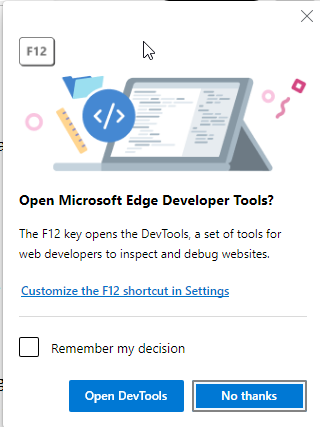
\includegraphics[]{edge_F12.png}
	\caption{F12 Debugging functie Microsoft Edge}
	\label{fig:EdgeF12}
\end{figure}
Klik op Open DevTools (eventueel kan je aanvinken dat Microsoft deze keuze moet onthouden).

Daarna kom in de Developer Tools terecht. Je krijgt dan naast de website die je bezoekt een uitgebreidde debugging tool zoals weergegeven in figuur \ref{fig:EdgeDebugger}.
\begin{figure}[h]
	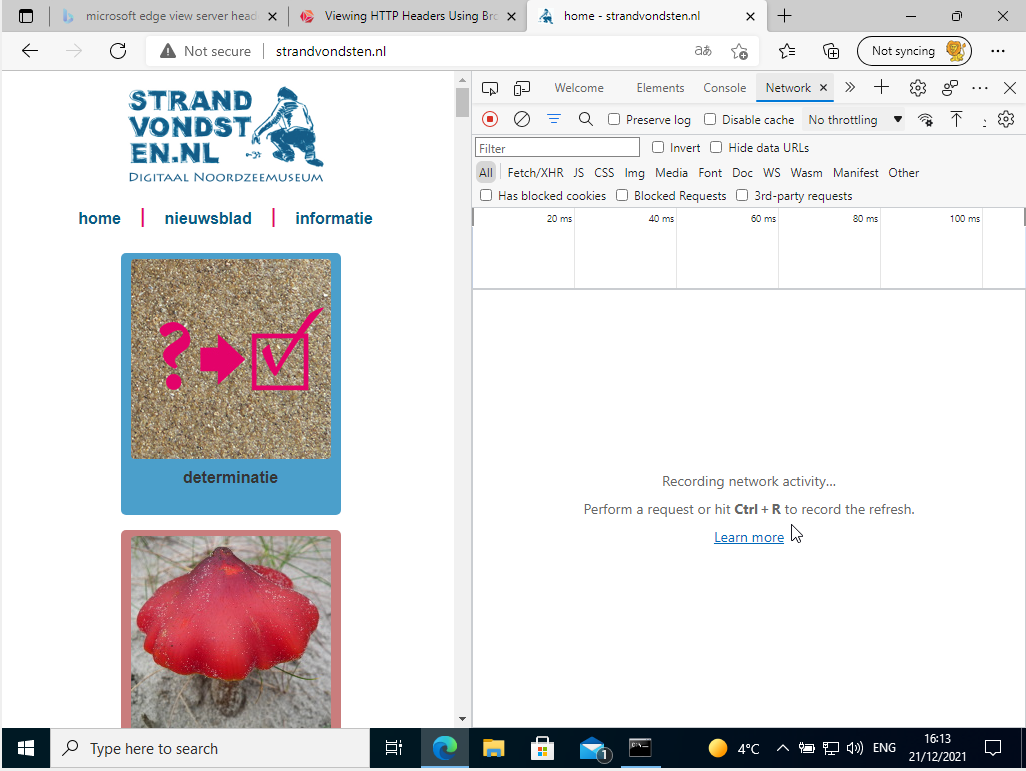
\includegraphics[width=0.9\linewidth]{Edge_Debugger.png}
	\caption{Microsoft Edge Developer Tools}
	\label{fig:EdgeDebugger}
\end{figure}


Selecteer in de balk met Welcome de Network tab en reload de pagina (aan de linker kant). Het scherm zal er dan ongeveer zo uit zien als in figuur \ref{fig:EdgeHeaders}.
\begin{figure}[h]
	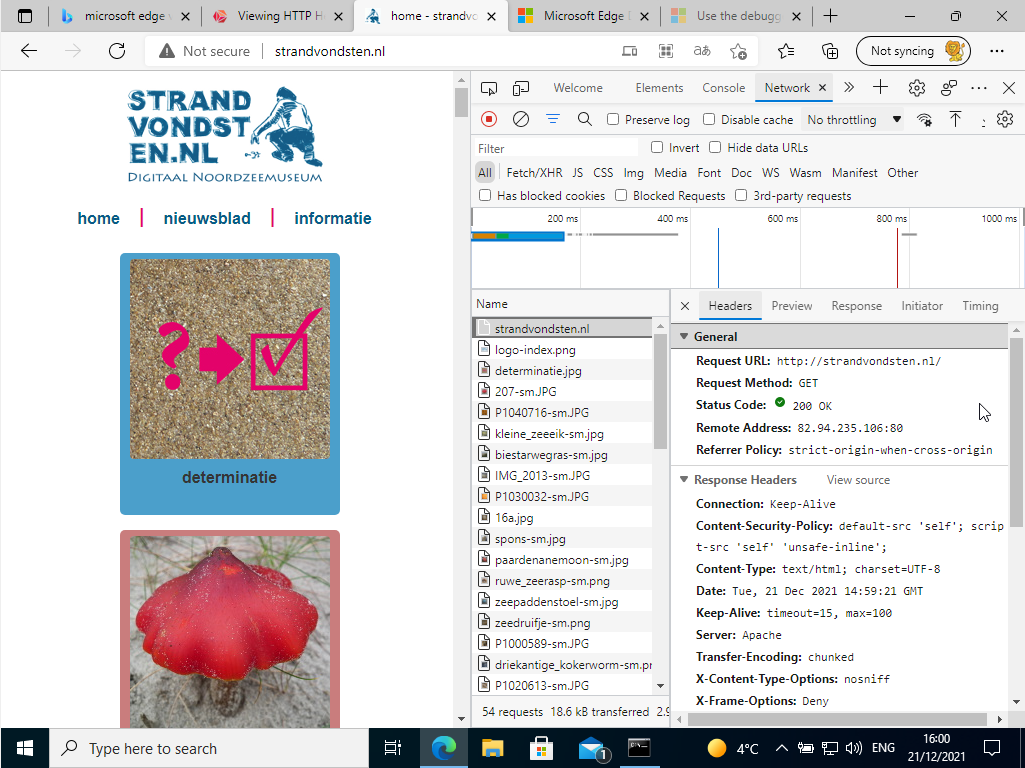
\includegraphics[width=0.9\linewidth]{Edge_Headers.png}
	\caption{Weergave van HTTP headers in Microsoft Edge}
	\label{fig:EdgeHeaders}
\end{figure}
Klik op het Headers tabblad en scroll aan de rechter onderkant helemaal omhoog en selecteer het bovenste element (in het voorbeeld: strandvondsten.nl), je ziet dan de headers die van de server terug zijn gekomen. Het zijn deze headers die van belang zijn in de rest van het document en die je op deze manier kan controleren.
